% vim: set tw=78 softtabstop=2 shiftwidth=2 et aw ai:
\documentclass{beamer}

\usepackage[utf8x]{inputenc}    % diacritice
\usepackage[romanian]{babel}
\usepackage{color}      % highlight
\usepackage{alltt}      % highlight

% highlight; comment this out in case you don't input code source files
%\usepackage{code/highlight}    % highlight

\usepackage{hyperref}      % folosiți \url{http://...}
          % sau \href{http://...}{Nume Link}
\usepackage{verbatim}

% Încărcăm simbolurilor Unicode românești în titlu și primele pagini
\PreloadUnicodePage{200}

\mode<presentation>
{ \usetheme{Berlin} }

\title[Intrumente colaborative]{Instrumente colaborative}
\subtitle{Dokuwiki, Git, Redmine}
\institute{ROSEdu Tech Talks}
\author[Răzvan Deaconescu]{Răzvan Deaconescu\\
  razvan@rosedu.org}
\date{5 martie 2011}

\begin{document}

% Slide-urile cu mai multe părți sunt marcate cu textul (cont.)
\setbeamertemplate{frametitle continuation}[from second]

% Arătăm numărul frame-ului
%\setbeamertemplate{footline}[frame number]

% Show contents at every section beginning. Ripped off from manual.
\AtBeginSection[] % Do nothing for \section*
{
  \begin{frame}<beamer>
    \frametitle{Cuprins}
  \tableofcontents[currentsection]
    \end{frame}
}

\frame{\titlepage}

\frame{\tableofcontents}

\section{Buzzwords}

\begin{frame}{Colaborare}
  \begin{itemize}
    \item mai multe entități (persoane, organizații) lucrează împreună
    \item obiective comune
    \item partajare (informații, resurse, cunoștințe)
    \item consens
    \item în general necesită coordonare/conducere/leadership
    \item cooperare -- țelurile pot diferi, doză de individualism,``side by
    side''
  \end{itemize}
\end{frame}

\begin{frame}{Instrumente colaborative}
  \begin{itemize}
    \item collaborative software
    \item ``how collaborative activities and their coordination can be
    supported by means of computer systems''
    \item ``the more people who use something, the more valuable it becomes''
    \item collaborative working environment
    \item virtual teams
  \end{itemize}
\end{frame}

\begin{frame}{Computer Supported Cooperative Work}
  \begin{figure}
    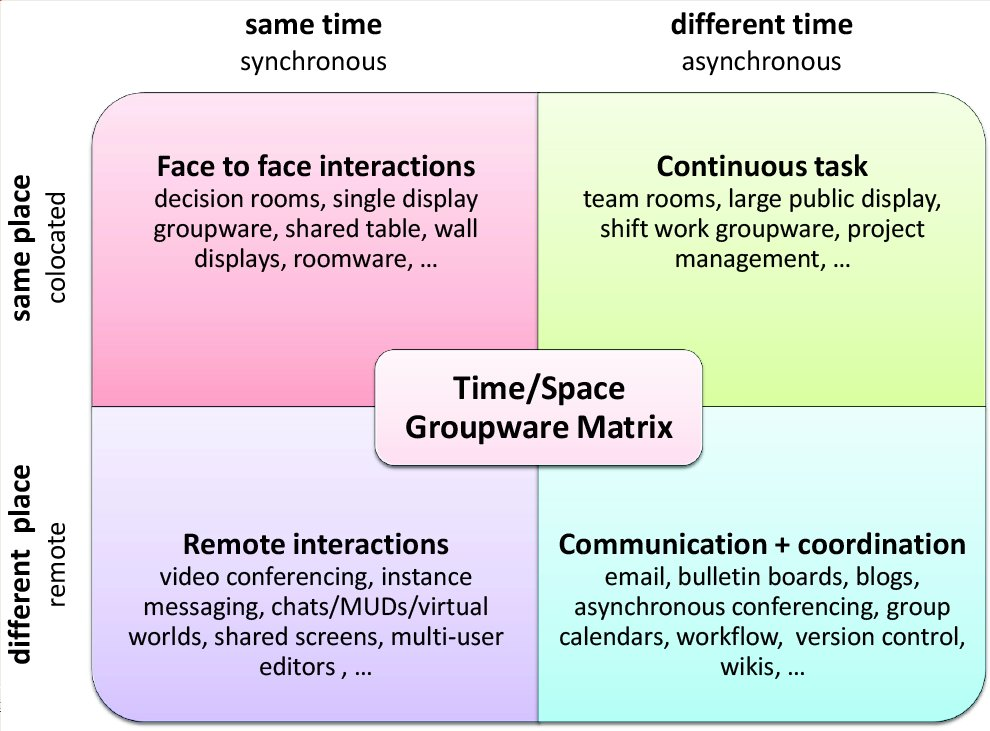
\includegraphics[scale=0.3]{img/cscw-matrix}
  \end{figure}
\end{frame}

\section{Instrumente colaborative}

\begin{frame}{Wikis}
  \begin{itemize}
    \item editare de conținut web
    \item sintaxă simplă
    \item generare rapidă de conținut
    \item colaborare facilă
    \item accent pe structură și conținut, mai puțin pe formă
    \item documentație, tutoriale, informare, proceduri
    \item MediaWiki, DokuWiki, TWiki, TikiWiki, MoinMoin, PmWiki
    \item \texttt{http://www.wikimatrix.org/}
  \end{itemize}
\end{frame}

\begin{frame}{Online Docs}
  \begin{itemize}
    \item colaborare în timp real
    \item integrare cu suite Office ``offline'' (upload, download)
    \item documente interne
    \item slide-uri, spreadsheets
    \item Google Docs, Microsoft Office Live, Oracle Cloud Office
  \end{itemize}
\end{frame}

\begin{frame}{VCS/SCM}
  \begin{itemize}
    \item Version Control System, Revizion Control System
    \item Source Code Management
    \item repository pentru cod
    \item colaborare între dezvoltatori
    \item commit-uri, ierarhie de commit-uri, istoric de modificări
    \item Git, Subversion, Perforce, Mercurial, Darcs, Bazaar
  \end{itemize}
\end{frame}

\begin{frame}{Mailing Lists/Forums/IRC/Usenet}
  \begin{itemize}
    \item discuții, întrebări, opinii, propuneri
    \item asincrone: liste de discuție, forumuri, Usenet, Google Groups
    \item sincrone: IRC, chat, video chat
    \item clienți de e-mail, clienți web, clienți IRC
  \end{itemize}
\end{frame}

\begin{frame}{Blogging}
  \begin{itemize}
    \item informare, tutoriale, comentarii
    \item asincrone
    \item în general folosite ca social software
  \end{itemize}
\end{frame}

\begin{frame}{File syncing/sharing}
  \begin{itemize}
    \item sincronizare/partajare a datelor
    \item sisteme de file-sharing
    \item rsync, Dropbox
  \end{itemize}
\end{frame}

\begin{frame}{DMS}
  \begin{itemize}
    \item Document Management System
    \item de obicei pentru instituții/companii
    \item colaborare, versionare, căutare, securitate, metadate
    \item folosit pentru documente digitale (scrise sau scanate)
    \item KnowledgeTree, Archivista, Alfresco
  \end{itemize}
\end{frame}

\begin{frame}{Calendaring}
  \begin{itemize}
    \item întâlniri, evenimente, task-uri
    \item invitații
    \item partajarea calendarului
    \item servere de calendaring (Open Calendar Server, Microsoft Exchange,
    Zimbra, bedework
    \item soluții online (Google Calendar)
  \end{itemize}
\end{frame}

\begin{frame}{LDAP/AD}
  \begin{itemize}
    \item Lightweight Directory Access Protocol / Active Directory
    \item stocarea informației într-un format de directoare (arbore):
    informații despre utilizatori, sisteme, contacte etc.
    \item folosit pentru autentificare unică
    \item OpenLDAP, Microsoft Active Directory
  \end{itemize}
\end{frame}

\begin{frame}{Groupware}
  \begin{itemize}
    \item soluție integrată
  \end{itemize}
\end{frame}

\begin{frame}{Software Project Management}
  \begin{itemize}
    \item soluție integrată
    \item wiki, ticket/issue trackers, repository, autentificare
    \item plugin-uri
    \item instalabile: Trac, Redmine, Launchpad, JIRA
    \item hosted: SourceForge, Google Code, CodePlex
  \end{itemize}
\end{frame}

\section{DokuWiki}

\begin{frame}{DokuWiki}
  \begin{itemize}
    \item TODO
  \end{itemize}
\end{frame}

\begin{frame}{De ce DokuWiki?}
  \begin{itemize}
    \item TODO
  \end{itemize}
\end{frame}

\begin{frame}{Când folosim DokuWiki?}
  \begin{itemize}
    \item TODO
  \end{itemize}
\end{frame}

\begin{frame}{Instalare și configurare}
  \begin{itemize}
    \item TODO
  \end{itemize}
\end{frame}

\begin{frame}{Cum se foloește?}
  \begin{itemize}
    \item TODO
  \end{itemize}
\end{frame}

\begin{frame}{Tips}
  \begin{itemize}
    \item TODO
  \end{itemize}
\end{frame}

\section{Git}

\begin{frame}{Git}
  \begin{itemize}
    \item TODO
  \end{itemize}
\end{frame}

\begin{frame}{De ce Git?}
  \begin{itemize}
    \item TODO
  \end{itemize}
\end{frame}

\begin{frame}{Când folosim Git?}
  \begin{itemize}
    \item TODO
  \end{itemize}
\end{frame}

\begin{frame}{Instalare și configurare}
  \begin{itemize}
    \item TODO
  \end{itemize}
\end{frame}

\begin{frame}{Cum se foloește?}
  \begin{itemize}
    \item TODO
  \end{itemize}
\end{frame}

\begin{frame}{Tips}
  \begin{itemize}
    \item TODO
  \end{itemize}
\end{frame}

\section{Redmine}

\begin{frame}{Redmine}
  \begin{itemize}
    \item TODO
  \end{itemize}
\end{frame}

\begin{frame}{De ce Redmine?}
  \begin{itemize}
    \item TODO
  \end{itemize}
\end{frame}

\begin{frame}{Când folosim Redmine?}
  \begin{itemize}
    \item TODO
  \end{itemize}
\end{frame}

\begin{frame}{Instalare și configurare}
  \begin{itemize}
    \item TODO
  \end{itemize}
\end{frame}

\begin{frame}{Cum se foloește?}
  \begin{itemize}
    \item TODO
  \end{itemize}
\end{frame}

\begin{frame}{Tips}
  \begin{itemize}
    \item TODO
  \end{itemize}
\end{frame}

\section{Concluzii}

\begin{frame}{Cuvinte cheie}
  \begin{columns}
    \begin{column}[l]{0.5\textwidth}
      \begin{itemize}
        \item TODO
      \end{itemize}
    \end{column}
    \begin{column}[l]{0.5\textwidth}
      \begin{itemize}
        \item TODO
      \end{itemize}
    \end{column}
  \end{columns}
\end{frame}

\begin{frame}{Resurse utile}
  \begin{itemize}
    \small
    \item TODO
  \end{itemize}
\end{frame}

\section{Întrebări}

\end{document}
